\documentclass[12pt, a4paper]{exam}
\usepackage{graphicx}
\usepackage[left=0.8in, top=0.7in, total={6.2in,10in}]{geometry}
\usepackage[normalem]{ulem}
\usepackage{comment}
\renewcommand\ULthickness{1.0pt}   %%---> For changing thickness of underline
\setlength\ULdepth{1.3ex}%\maxdimen ---> For changing depth of underline
\usepackage{hyperref}
\usepackage{url}
\usepackage{float}

\begin{document}
	%\thispagestyle{empty}
	\noindent
	\begin{minipage}[l]{0.1\textwidth}
		\noindent
		
\includegraphics[width=1.8\textwidth]{res/iiserb_logo.png}
	\end{minipage}
\hfill
\begin{minipage}[c]{0.8\textwidth}
	\begin{center}
		{\large	Indian Institute of Science Education and Research Bhopal \par
		\large	\par
	\large \textbf{	Computer Vision( DSE/EECS-312)}	\par
Bonus Assignment-1}
	\end{center}
\end{minipage}
\par
\vspace{0.2in}
\noindent
\uline{Deadline: 14-10-2024, 11:59 PM	 \hfill 		\hfill Max mark: 10} \\
\uline{Please follow the instructions carefully.}
\par 
\vspace{0.15in}
\noindent
\centering
{\small \bfseries \begin{enumerate}
\item Plagiarism and copying from anywhere (similar submission) can debar you from this course and invite the academic dishonesty policy.
    \item The length of the video should be between 3-5 minutes.
    \item The video should not be abusive and/or harmful in any sense to anyone.
    \item The purpose is to learn the recent advancements of AI in the Computer vision world only. Therefore, no personal interest will be entertained. \\
 \end{enumerate}   
    
   \textbf{Submission:}\\
  \begin{enumerate}
    \item Video
    \item A 1-2 page report only in the given overleaf template explaining the topic of your video, the crux, an explanation of the tool used in both questions and its link.
    
\end{enumerate}}
\vspace{0.2in}
\begin{questions}

	\pointsdroppedatright
	\question Using recent advancements in generative AI and computer vision technologies, create a simulated debate video featuring two prominent historical or contemporary figures. The debate should center around a critical and timely issue, such as climate change, technological ethics, international relations, or social justice. Additionally, consider the ethical implications and technical challenges of creating realistic AI-generated representations of real individuals.

 Here is one example: \url{https://www.linkedin.com/feed/update/urn:li:activity:7118570023987683328?updateEntityUrn=urn%3Ali%3Afs_feedUpdate%3A%28V2%2Curn%3Ali%3Aactivity%3A7118570023987683328%29} \\
 
\vspace{0.2in}
\textbf{Answer:}

I used several tools to create it. First I generated the script using ChatGPT, then I used Verbo ai to generate a video from the face given. Then I used media.io and fakeyou.com to generate the audio for each individuals. Then I finally combined the videos using video editing tool Davinci Relove. The individuals are Leonel messi and Donald trump. The topic of the debate is "Leading world towards AI". The video has been attached.

\newpage

\vspace{0.2in}
    \pointsdroppedatright
	
	\question Explore the various open-source toolboxes and applications used in the field of computer vision and come up with some interesting applications or toolboxes related to the Computer Vision field (Inpainting, Pose Estimation, DeepFakes(Image, Audio or Video), Adversarial Example Generation, Style Transfer). Select any toolboxes or applications and use them to test their effectiveness in solving the specific problem you are addressing, and discuss their core functionalities, advantages, and real-world applications.\\
\vspace{0.2in}
\textbf{Answer:}

Recently, I was working on the project of ai gym trainer. So what you do is basically, record your vedio or turn on your camera for live rep counting. So follow is the idea:

The problem statement is simple, given a video, I have to count the number of reps user has performed and also check if the form of the user is correct or not. I have to do this in real time too, since I want to support video to from live vedio feed.

\textbf{Mediapipe}

I discovered this library, which is developed and maintained by Google. I used it to extract. To discuss on some of the core functionalities of mediapipe library, below image describes number of features that this library has.

\begin{figure}[H]
    \centering
    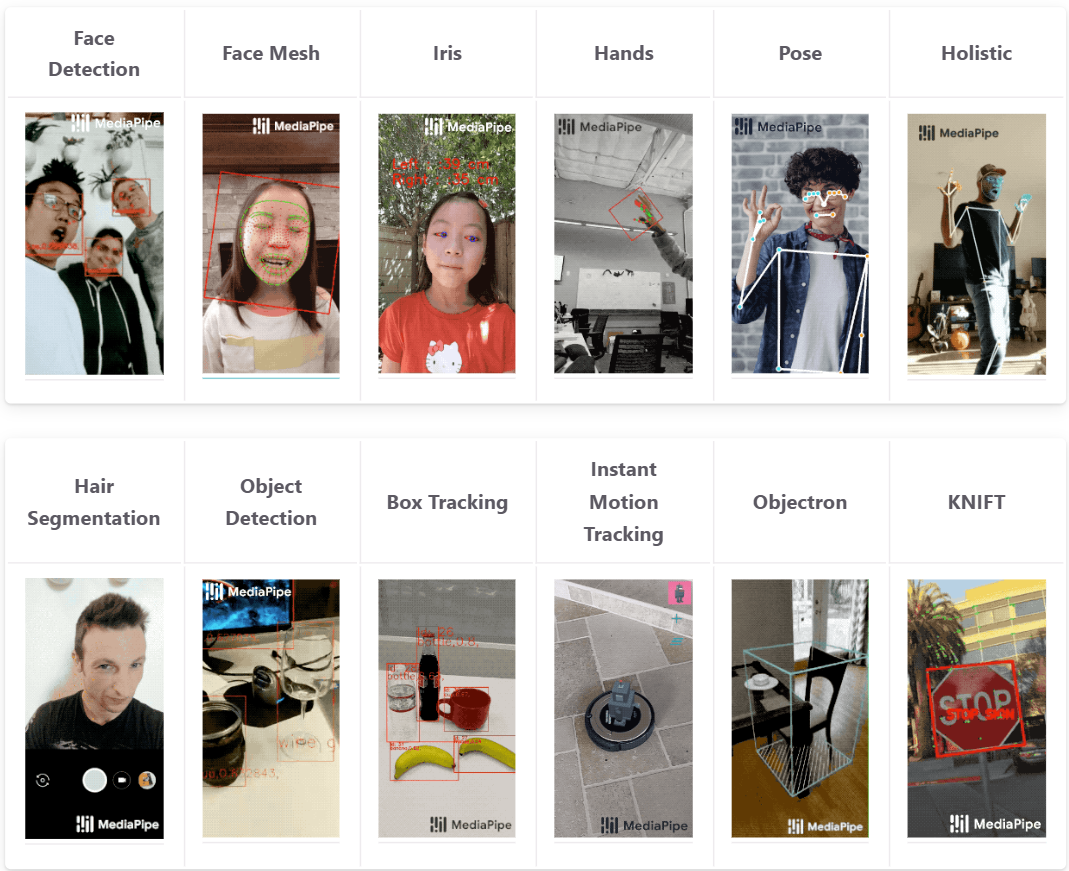
\includegraphics[width=1.06\textwidth]{res/Mediapipe.png}
    \caption{Mediapipe features}
    \label{fig:2_mediapipe}
\end{figure}


\textbf{mediapipe}

I used it to extract skeleton of the human body currently in frame. This is a pose estimation problem


\begin{figure}[H]
    \centering
    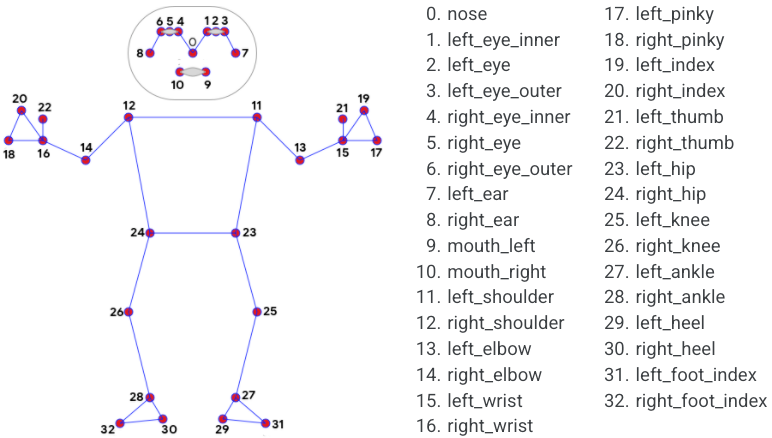
\includegraphics[width=1.06\textwidth]{res/pose_tracking_full_body_landmarks.png}
    \caption{Pose tracking full body landmarks}
    \label{fig:2_mpose_landmarks}
\end{figure}

I then used the extracted skeleton to extract the angles of the joints. I used these angles to figure if the angles cross certain threshold to count the rep. I also used the angles to figure out if the form of the person is correct or not.

I haved added a screenshot of working of that project.

\begin{figure}[H]
    \centering
    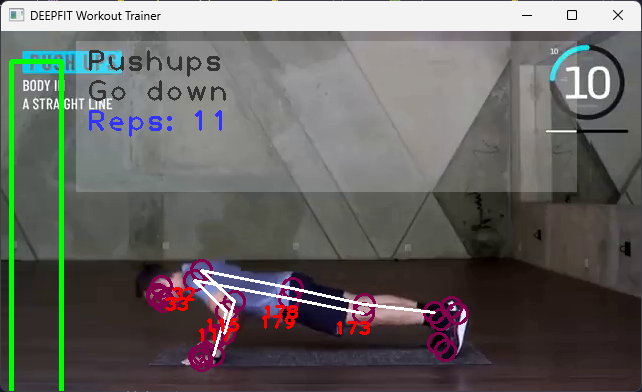
\includegraphics[width=.8\textwidth]{res/deepfit.png}
    \caption{AI gym trainer app}
    \label{fig:2_deepfit}
\end{figure}

\vspace{0.2in}


\end{questions}

\end{document}